\textit{}\chapter{Methodology: Wicked Problems}
\label{chapterlabel5}

\section*{Chapter summary}

In this chapter I will introduce the empirical methodology for this exploratory research. A mix of existing cross-disciplinary approaches have been applied, for instance, research-through-design or non-linear iterative urban prototyping. The aspects I will focus on are of \textit{technical}, \textit{social} and \textit{spatial} nature.  I will further introduce a technology that allows people to express their sentiments in public and layout the cases in which this technology has been used.  \newpage

%%%%%%%%%%%%%%%%%%%%%%%%%%%

\section{Research through Media Architecture: A non-linear approach}

%Literature:
%Marshall, P., et al.: Using F-formations to analyse spatial patterns of interaction in physical environments. In: Proceedings of CSCW, pp. 445–454. ACM (2011)
%John Zimmerman, Jodi Forlizzi, Shelley Evenson, Research Through Design as a Method for Interaction Design Research in HCI

Designing interactive systems for social interactions is considered to be a "wicked problem". Which means that we will not find a perfect solution/answer to the question, but by addressing it we will find out more about the "problem" itself and may be able to suggest possible solutions through explorational studies (G. Fitzpatrick' The Locales Framework: Understanding and Designing for Wicked Problems )

As mentioned in the background section our definition for architecture derives from practice. Media Architectures manifest the idea of incorporating media systems already into the initial design process. In other words, Media Facades embed electronic surfaces, but Media Architectures embody multi-dimensional media systems. 

This PhD research is located within the fields of architecture and human-computer interaction in urban space (urban HCI) both applied and theoretical. 
Both fields benefit from each other in their work from understanding human behaviours and social interactions in urban space, which are increasingly mediated through digital media technologies such as \textit{Urban Screens} or \textit{Media Architecture}.

We explore, how one may design for interactions with temporary large electronic surfaces through examining the \textit{technical}, \textit{spatial }and \textit{social} aspects in each of the conducted studies. In order to answer this question we observe emerging practices, human behaviours and interactions around such media interventions and their relationship to the properties of public space. 
A methodology has been developed, which brings together empirical methods from architecture, architectural research and interaction design research (O’Neill et al., 2006; Fatah et al, 2013). 
This research is mainly driven by a research-through-design approach incorporating qualitative and quantitative methods.
Within the scope of this research we iteratively design, prototype and implement a series of temporary media installations that involve Media Architectural Interfaces (MAI).
We engage and negotiate with museums, universities, media art festivals and large corporates to place our projects.
We evaluate mediated public interactions around the temporary media installation with regard to the properties of the given public space and compare our findings with existing socio-spatial interaction frameworks.


When designing for interactions with temporary media architectural installations we focus on the following three aspects:

%%%%%%%%%%%%%%%%%%%%%%%%%%%

\begin{itemize}
\item \textit{\textbf{technical}} - what is needed to design and implement interactive systems (i.e. technology, skills, dealing with stakeholders, curators, competitions)
\item \textit{\textbf{spatial}} - describing and understanding the spatial requirements that constitute public spaces for interactions
\item \textit{\textbf{social}} - describing and understanding of emergent human behaviours and social interactions and experiences with interactive systems 
\end{itemize}

%%%%%%%%%%%%%%%%%%%%%%%%%%%

The methodology has four objectives in order to address the research questions: 
\begin{enumerate}
\setcounter{enumi}{0}
\item \textbf{\textit{Designing and implementing iteratively}} a series of projects that involve MAI.
\item \textit{\textbf{Capturing and analysing}} social behaviours and interactions of participants interacting with the projects. 
\item \textbf{\textit{Relating}} identified behaviours and interactions of participants to the given spatial context.
\item \textbf{\textit{Matching}} socio-spatial observations with existing spatial interaction frameworks.
\item \textbf{\textit{Generalising}} the findings in a proposed taxonomy following the suggested MAI framework.
\end{enumerate}

%%%%%%%%%%%%%%%%%%%%%%%%%%%

Eventually the aim is to give guidance to architects, designers, urban planners, curators and artists on where to best position interactive systems to leverage the experience of city dwellers and to support social interactions.  

%%%%%%%%%%%%%%%%%%%%%%%%%%%

\begin{itemize}
\item iterative as we continuously advanced the \textit{Interface} and aimed to approach various kinds of surface typologies
\item non-linear as we were limited in the opportunities to deploy our \textit{Interface}. We had to apply for several opportunities such as media art festivals in order to get access to different kinds of architectural surface. For example we got the opportunity to implement our ideas at a Media Facade (i.e. SAOP) before actually being able to explore Urban Screens (i.e. RIGA) 
\item flexibility to constantly adapt to unexpected opportunities or changes either in event, competition, curation, location, technology or caused by the user (Reid et all, 2005; Briones, 2006; Kukka et all, 2010)
\end{itemize}

%%%%%%%%%%%%%%%%%%%%%%%%%%%

Speculative Design

This PhD is not about problem solving it is about envisioning a future where technology serves our desires.

"Rather than giving up altogether, though, there are other possibilities
for design: one is to use design as a means of speculating how things could
be—speculative design. This form of design thrives on imagination and aims to
open up new perspectives on what are sometimes called wicked problems, to
create spaces for discussion and debate about alternative ways of being, and
to inspire and encourage people’s imaginations to flow freely. Design
speculations can act as a catalyst for collectively redefining our relationship
to reality."

"In Speculative Everything, Anthony Dunne and Fiona Raby propose a kind of design that is used as a tool to create not only things but ideas. For them, design is a means of speculating about how things could be—to imagine possible futures. This is not the usual sort of predicting or forecasting, spotting trends and extrapolating; these kinds of predictions have been proven wrong, again and again." From the book: Speculative Everything Design, Fiction, and Social Dreaming By Anthony Dunne and Fiona Raby

%%%%%%%%%%%%%%%%%%%%%%%%%%%

Tools

Not only the decrease in cost for computer technology but also the accessibility to computational tools such as Processing (source) or Arduino (source) allowed other disciplines to explore and involve ICTs into their practices. More recently visual programming such as vvvv (source) or grasshopper (source) further lowered the barriers for non-programmers to apply computational methods and tools for their purposes. In this respect the course in Adaptive Architecture and Computation at the Bartlett School of Architecture is to mention as a source for interdisciplinary education of designers, architects and urban planners (source).   

%%%%%%%%%%%%%%%%%%%%%%%%%%%

Hacking and DIY Culture

- art, design and architecture are currently benefiting from the open-source and hacking communities 

%%%%%%%%%%%%%%%%%%%%%%%%%%%
Media Art and Temporary Installations as a Methodology 

"Temporary installations create engaging environments over a limited period
of time, while offering the opportunity to test concepts and prototypes in a
real-life setting. A temporary realisation of a project can proof a concept with
hard facts, or highlight areas that require improvement and refinement. Success
or failure can be assessed, and economic, social, environmental and other
benefits evaluated and clearly demonstrated. As test-bed for potential permanent
installations, temporary projects are particularly interesting for the realisation of
more innovative and experimental proposals, likely to be rejected by decision-makers. Lighting festivals are particularly relevant in this area."
acknowledged by Arup: ARUP, Cities Alive - Rethinking the Shades of Night. 

%%%%%%%%%%%%%%%%%%%

Identifying the limitations of your research

Designing means knowing your limitations and constraints. This is a finding that applies to architectural designing and designing for interactions.

%%%%%%%%%%%%%%%%%%%%%%%%%%%

\section{The case study}
We demonstrate and analyse how temporary media architectural installations might entice people to step out of their daily routines in public spaces. This is achieved through a series of design studies, which can be summarised as {A Field Trip into Sentiment Architectures}. 
The idea of \textit{A Field Trip into Sentiment Architectures} is an applied research into situated and shared interfaces in public space that aim to bring together people through giving them the ability to collectively share and project their emotions in public space. The field trip started some time ago with the \textit{Swipe I like} (SIL) project and the \textit{Sentiment Cocoon} is the most advanced prototype so far \label{study_overview}. In the following we give an overview of the studies carried out and briefly summarise the aims and objectives of each study. 

%%%%%%%%%%%%%%%%%%%%%%%%%%%

\begin{table}[h!]
\centering
\resizebox{\textwidth}{!}{
\setlength{\extrarowheight}{8pt}
\begin{tabular}{ccccccc}
\multicolumn{7}{c}{Field trip into Sentiment Architectures} \\ \hline
\multicolumn{2}{c|}{\textit{Pre-Study}} & \multicolumn{3}{c|}{\textit{Study I}} & \multicolumn{2}{c}{\textit{Study II}} \\
\multicolumn{2}{c|}{\textbf{Swipe I like}} & \multicolumn{3}{c|}{\textbf{Smart Citizen Sentiment Dashboard (SCSD)}} & \multicolumn{2}{c}{\textbf{Sentiment Cocoon (SC)}} \\ \hline
\multicolumn{1}{c|}{SIL} & \multicolumn{1}{c|}{VEIV} & \multicolumn{1}{c|}{RIGA} & \multicolumn{1}{c|}{SAOP} & \multicolumn{1}{c|}{LINZ} & \multicolumn{1}{c|}{ARUP} & VIVID \\ \hline
\multicolumn{1}{c|}{\textit{-}} & \multicolumn{1}{c|}{\textit{DIY display}} & \multicolumn{1}{c|}{\textit{Urban Screen}} & \multicolumn{1}{c|}{\textit{Media Facade}} & \multicolumn{1}{c|}{\textit{Media Architecture}} & \multicolumn{1}{c|}{\textit{Media Architecture}} & \textit{Media Architecture}
\end{tabular}
}
\caption[Overview of conducted design studies]{Overview of conducted design studies including the types of electronic surfaces.}
\label{study_overview}
\end{table}

%%%%%%%%%%%%%%%%%%%%%%%%%%%

The following aims and objectives have been defined:

\begin{singlespace}{

\begin{labeling}{projects}

\item [\textbf{SIL}] 
\begin {itemize} 
\footnotesize
\item [\textit{aims}] Enhancing engagement and revealing emergent social behaviours through implementing novel digital technologies in public space. 
\item [\textit{objectives}] Designing and implementing a novel tangible interface (i.e. physical \textit{I like} button) in public space that lets people share their sentiments with their digital networks.

\end{itemize}

\item [\textbf{VEIV}] 
\begin {itemize}
\footnotesize
\item [\textit{aims}] Providing immediate visual feedback to participants engaging with novel tangible interfaces.
\item [{objectives}] Connecting physical {I like} button to a large electronic surface (i.e. {DIY display} )in public space to provide users with immediate visual feedback.
\end{itemize}

\item [\textbf{RIGA}] 
\begin {itemize}
\footnotesize
\item [\textit{aims}] Exploring the effect of the positioning of large electronic surfaces on the existing flow of people in urban space.
\item [{objectives}] Design iteration of tangible interface (i.e. {Sentiment Dashboard}) and careful positioning of the {Sentiment Dashboard} and the attached electronic surface (i.e. {Urban Screen}) in urban space.
\end{itemize}

\item [\textbf{SAOP}]
\begin {itemize}
\footnotesize
\item [\textit{aims}] Exploring up to what scale the designed interactive system works in terms of human behaviour and social interactions.
\item [\textit{objectives}] Connecting the the \textit{Sentiment Dashboard} to a large existing \textit{Media Facade}. 
\end{itemize}
 
\item [\textbf{LINZ}] 
\begin {itemize}
\footnotesize
\item [\textit{aims}] Exploring the ambient character of large electronic displays and the appearance of Media Architecture during day and night and its effect on human behaviours and social interactions.  
\item [\textit{objectives}]Connecting the the \textit{Sentiment Dashboard} to a large existing three dimensional \textit{Media Architecture}.
\end{itemize}

\item [\textbf{ARUP}]
\begin {itemize}
\footnotesize
\item [\textit{aims}] Designing and implementing of temporary \textit{Media Architecture} based on the findings from previous studies.  \newline Incorporating the process of fabrication in public to explore social interactions. \newline Exploring the longitudinal effects on interactions of media architectural systems.
\item [\textit{objectives}] Collaborating with a large team of engineers and designers to implement our design of a self fabricated \textit{Media Architecture}.
\end{itemize}

\item [\textbf{VIVID}] 
\begin {itemize}
\footnotesize
\item [\textit{aims}] Designing and implementing a different temporary \textit{Media Architecture} with a novel tangible interface in a public outdoor space to confirm our previous findings.
\item [{objectives}] Designing and implementing a different tangible interface (i.e.{Palm Pulse Reader}). 
\end{itemize}

\end{labeling}
}
  
  \end{singlespace}



As outlined in the framework (section link), the Media Architectural Interface (MAI) consists out of two components: 
The \textit{Interface} is a situated an shared ‘tangible user interface’ that generates user specific data, whilst the \textit{Surface} is the component that displays the data generated through the \textit{Interface}. 
The \textit{Surface} might be a facade with a building projection, an urban screen, or a media facade and might change in its size or materiality depending on the location of the case study. 

Only the appearance (i.e. case or description) might change according to the content of the deployment (\label{interfaces}).
\begin{itemize}
\item the aim was to invent a interactive system that identifies every single user and her vote to be able to identify patterns of behaviour
\item At the same time the affordance (reference) of the physical device needs to be well designed and its use as little time consuming as possible - otherwise people would not use it.
\end{itemize}

\begin{figure}[!h] 
\centering
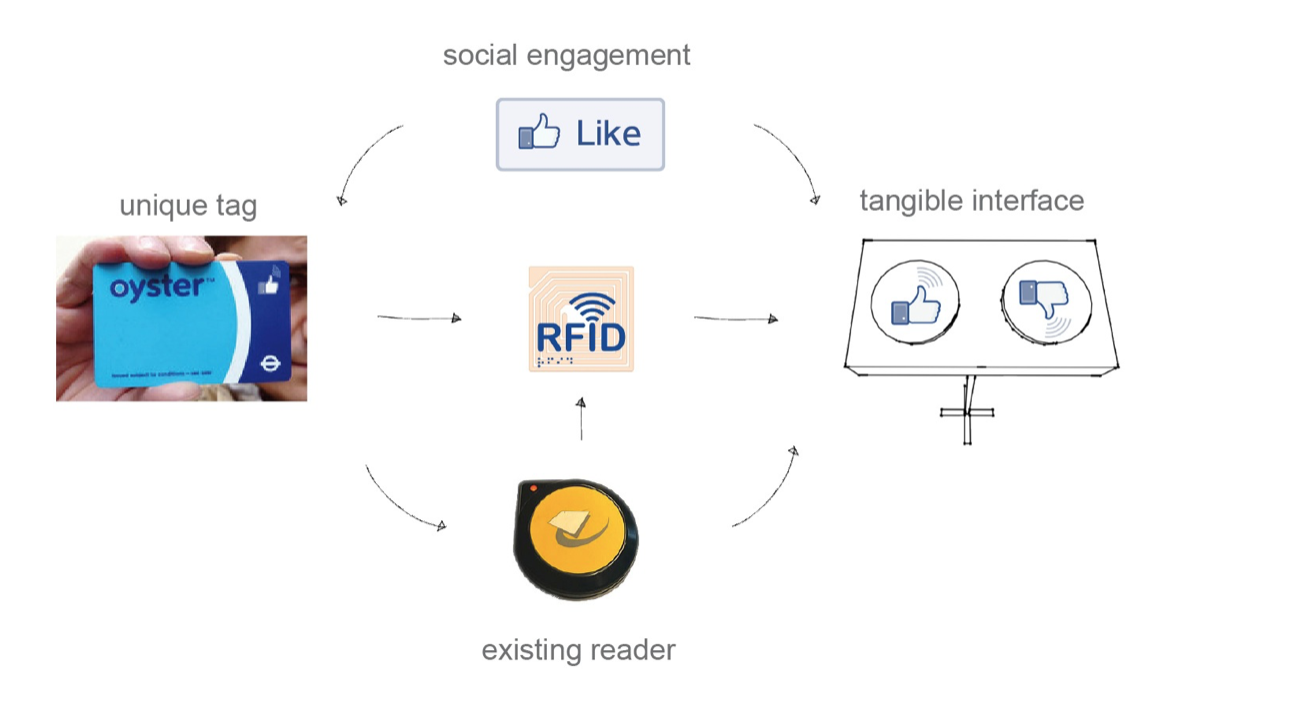
\includegraphics[width=\textwidth]{Illustrations/InteractionConcept.png}
\caption [Interaction design concept] {Concept of linking RFID technology with a tangible interface. }
\label{interfaces}
\end{figure}


\subsection{The Interface}

\begin{figure}[!h] 
\centering
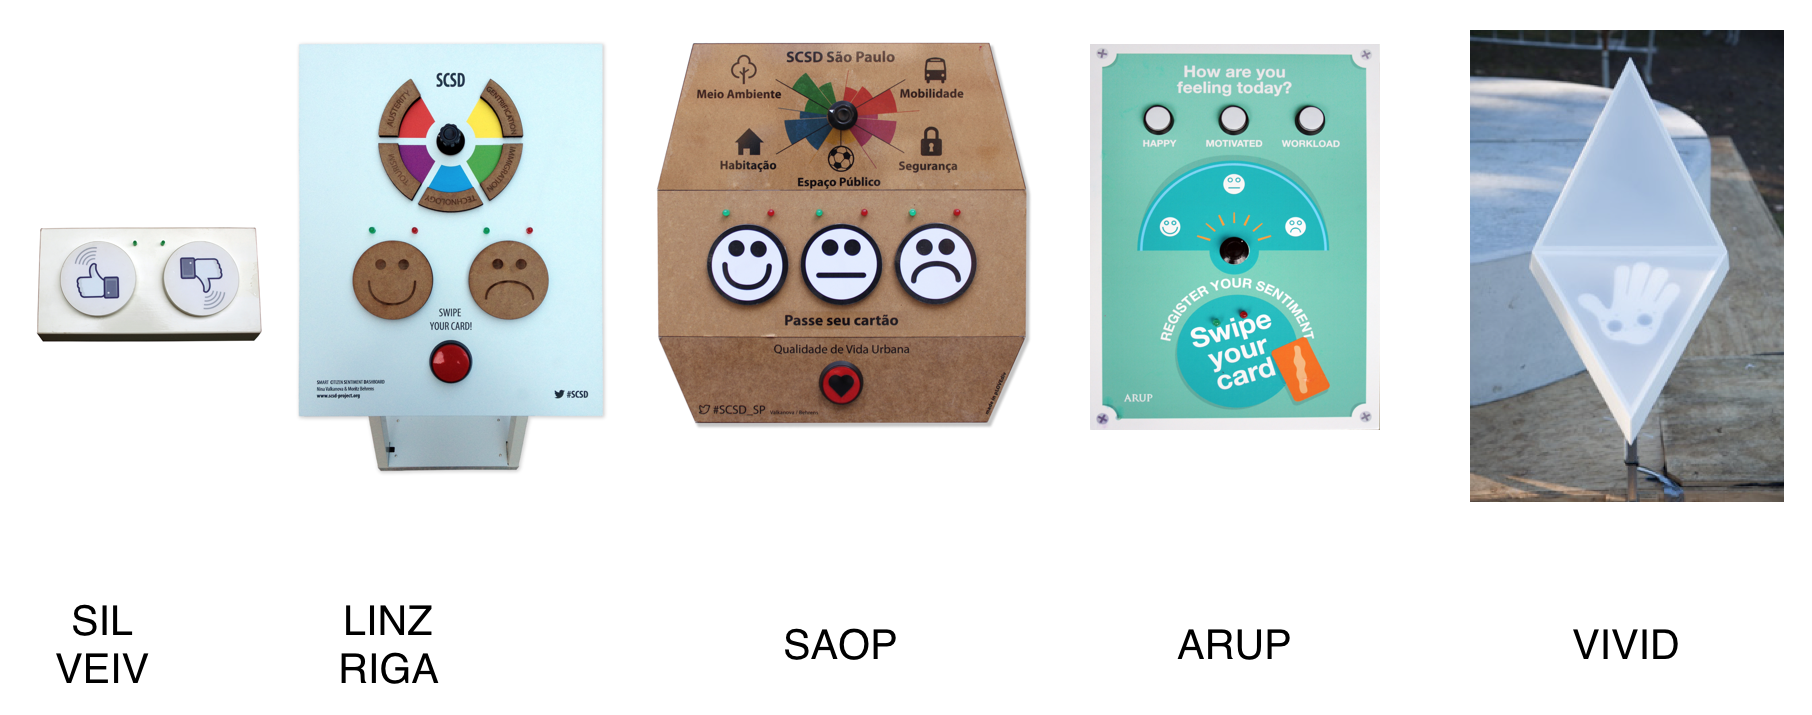
\includegraphics[width=\textwidth]{Illustrations/Interfaces.png}
\caption [Tangible User Interfaces] {Five different \textit{Interfaces} as used during the case studies.}
\label{interfaces}
\end{figure}

For this research the shared \textit{Interface} consists of an interactive system that has been iteratively designed, developed and implemented during several trial studies as part of my MSc studies in Adaptive Architecture and Computation at UCL The Bartlett (i.e. Behrens, 2011; Behrens, 2013). 
The system architecture is intended to make use of ubiquitous plastic smart cards, such as the public transport card for  London called Oyster Card. The technology behind these cards involves radio-frequency identification (RFID), which mostly consist of passive Mifare 13,56 MHz RFID microprocessors equipped with an antenna laminated into the plastic cards.
Latest research on RFID suggests that this widespread technology is not only suitable for logistic and security purposes, but emerges in applications that (ob-) serve our everyday life (Arnall 2009).

We aimed to build on the fact that almost every citizen is carrying around such an identifiable tag in form of a travel card, a building access card or any other card distributed for digital identification.
The idea is to make use of the existing smart technology beyond travel or access purposes and allow citizens to express their mood and opinion instantly using this technology in the urban realm. 

Their broad dispersal is a major advantage and positively affects the accessibility and affordance of the ‘I Like’ system. 
Swiping this card became a common use and is another benefit for our project.

Having this in mind the technology and its current use fits well into the underlying idea of making technology shared and situated for everyone in public space. 


\subsection{The Surface}

\begin{figure}[!h] 
\centering
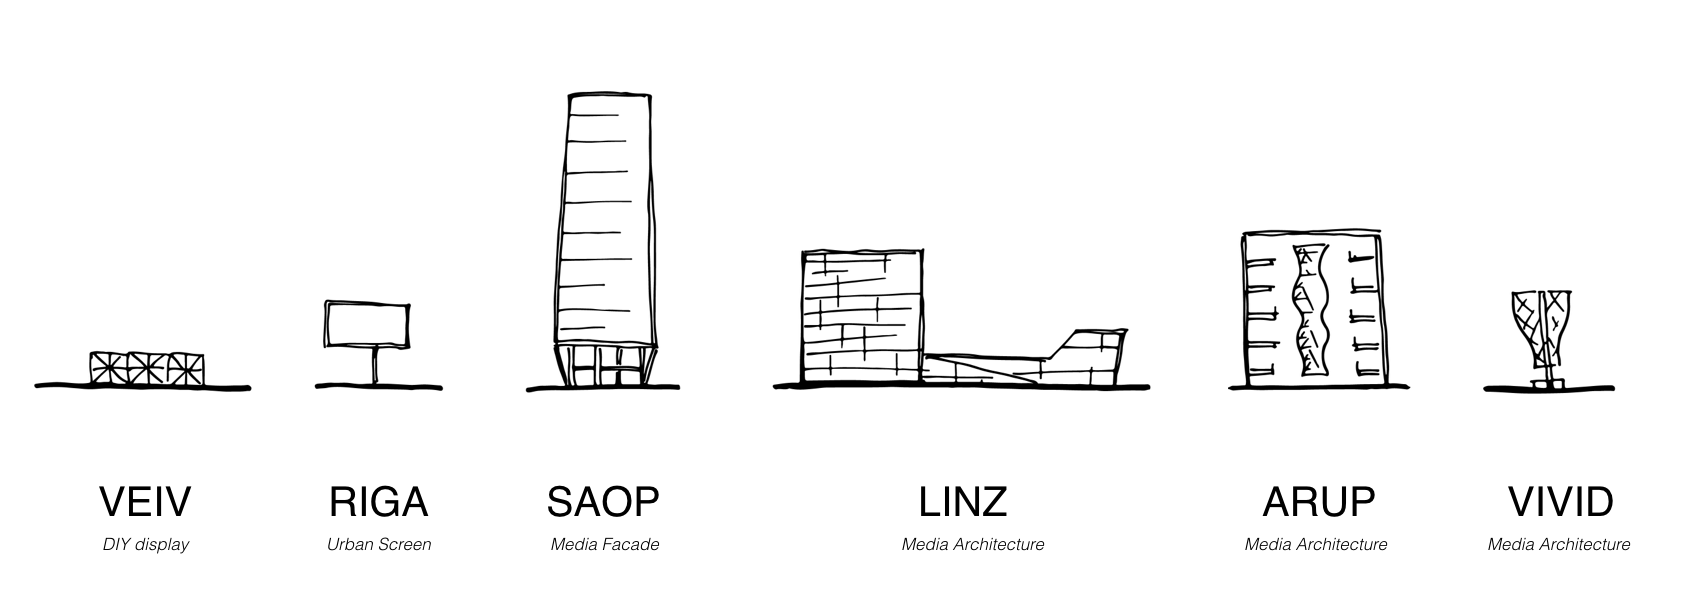
\includegraphics[width=\textwidth]{Illustrations/Surfaces.png}
\caption [Typology of architectural surfaces] {Typology of five different \textit{Surfaces} as used during six case studies.}
\label{surfaces}
\end{figure}


\subsection{The Context}



\section{Data collection, observations and analysis}

Using an RFID tag will allow to gather data (fig. 6) such as preference of interactions (1), identification of interaction (2), date (3), and time (4) of interactions.

\begin{figure}[!h] 
\centering
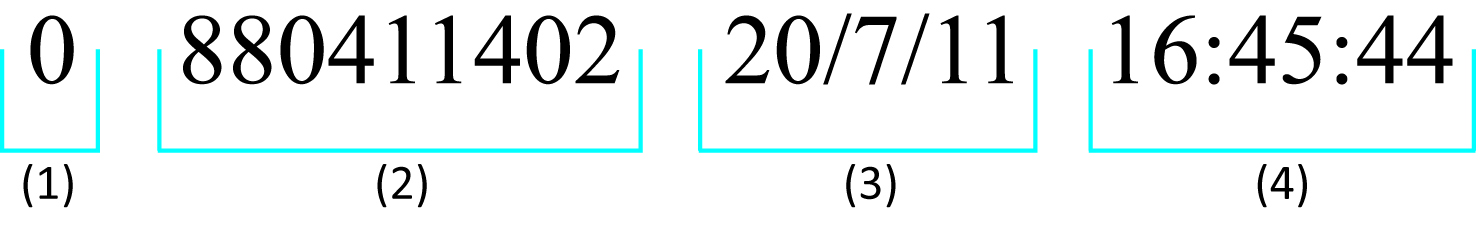
\includegraphics[width=\textwidth]{Illustrations/numbers.jpg}
\caption [Data structure] {Using an RFID tag will allow to gather the following data: preference of interactions (1), identification of interaction (2), date (3), and time (4) of interactions.}
\label{Numbers}
\end{figure}

The TUI is connected to a database, which logs all data. 
The visualization for the carrier will pick up the data from the database. 
Interactions with the feedback device will be plotted quantitatively onto timeline diagrams, which show the ID number of the participants transport card, the time when the interaction took place and the preference of the interaction (i.e. like or dislike).
The outcomes of the surveys will be visualized and qualitative observations and interviews will be summarized in written form.
